% !TEX root = ../utltcp-paper.tex


% Having identified the requirements in the previous section, we now present the
% overall TCP Hollywood architecture, and design of the wire protocol.

TCP Hollywood has been designed to be deployable on the ossified Internet
as it exists today, and to support partial deployments where only the sender
or the receiver has been upgraded to support the TCP Hollywood extensions.
The nature of the extensions we propose supports the former, while the
latter is achieved by splitting the functionality between a user-space
intermediary `shim' layer and a set of extensions to the kernel TCP stack.
The intermediary layer operates over either unmodified TCP, or with the
TCP Hollywood kernel extensions enabled. The user and kernel components
are represented in the overall architecture represented in Figure
\ref{diagram:architecture}. In discussing the architecture it is useful to
consider the sender separately from the receiver, and for each to consider
the user-space intermediary layer separately from the kernel TCP extensions.

\begin{figure}[t]
	\centering
	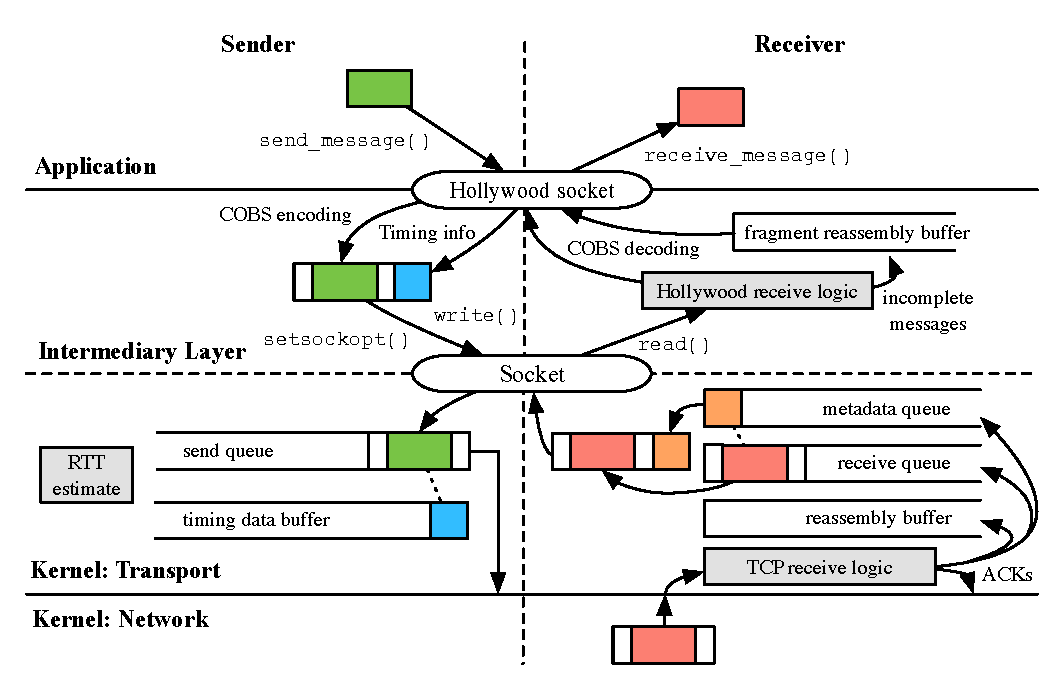
\includegraphics[width=\columnwidth,height=2.2in]{figures/message-flow-combined.pdf}
	\caption{TCP Hollywood sender and receiver architecture}
	\label{diagram:architecture}
\end{figure}

%--------------------------------------------------------------------------------------------------
\subsection{TCP Hollywood Sender architecture}
\label{subsec:sender}

The architecture of a TCP Hollywood sender is shown in the left hand side
of Figure~\ref{diagram:architecture}. The sender inherits the requirements
identified in Section~\ref{sec:background} to support a timed,
message-oriented, transport abstraction, with inconsistent retransmissions.
%This is supported by the user-space intermediary layer, and an optional
%(but highly desirable) set of changes to the in-kernel TCP sender.

The intermediary layer provides the message-oriented abstraction. It accepts
a sequence of messages (i.e., datagrams, rather than a byte stream) from the
application, with optional timeliness and dependency information,
to be delivered to the destination.
%
% For those messages that have no timeliness or dependency requirements,
%
The intermediary layer supports a sub-stream abstraction, allowing messages from multiple flows
to be multiplexed on a single transport-level connection (similar to how multiple streams
can be sent within a single SCTP association \cite{rfc:4960}).  This can
be used to cleanly multiplex audio and video flows onto a single
connection, or to distinguish multiple layers of a stream encoded using
scalable video coding~\cite{Ohm05}, for example using H.264/SVC.
%
The intermediary layer appends a sub-stream identifier to messages before
they are encoded, framed, and passed to the kernel TCP sender, with a
default sub-stream being reserved for flows where no sub-stream is
specified.  The application can provide timing or dependency data via
the intermediary layer API. This is passed to the kernel alongside the
encoded message, and used to determine whether inconsistent
retransmissions are appropriate.

To support a message-oriented abstraction over a TCP byte stream, the
TCP Hollywood flows must be resilient to re-segmentation or segment coalescing
by middleboxes. Message integrity must be protected: messages received
must have been sent, and only complete messages must be delivered.  This
is ensured by the intermediary layer, which frames messages with a leading
and trailing marker. The effect is shown in Figure~\ref{diagram:resegmentation},
where markers can be used to delineate messages irrespective of the
segmentation. The intermediary layer encodes messages with consistent overhead
byte stuffing (COBS)~\cite{CB97COBS}; this efficiently encodes the stream
to escape all zero bytes, allowing their use as framing markers, while still
providing a transparent channel that can carry any message.

The TCP sender implementation in the kernel is modified to perform
consistent segmentation, and to manage inconsistent retransmission
by tracking message timing, deadline expiration, and dependencies.
Consistent segmentation ensures that a single \texttt{write()} call made
by the intermediary layer will generate a single TCP segment, provided the
size of the segment does not exceed the MTU.
This ensures each message is sent in a separate TCP segment, allowing the
receiver to process it independently of other messages, reducing latency.
This implies disabling Nagle's algorithm (i.e., setting
the \texttt{TCP\_NODELAY} socket option) to avoid unnecessary buffering --
Nagle's algorithm would not provide a significant benefit to our target
applications, where messages are large compared to their headers.

\begin{figure}[t]
 \centering
 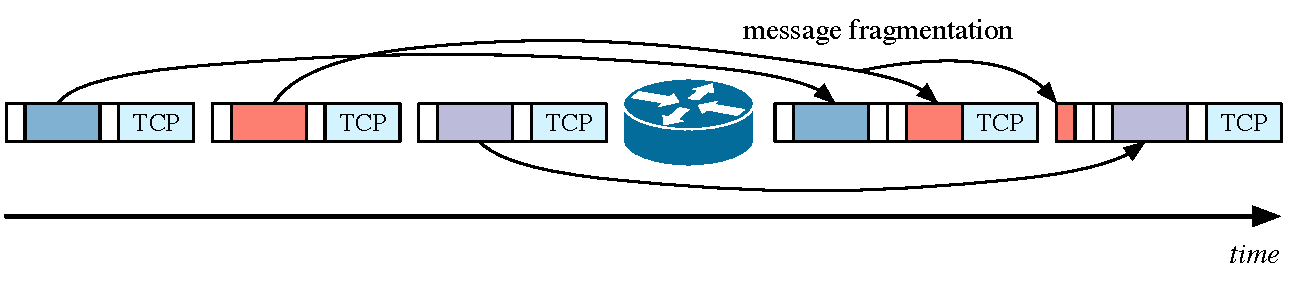
\includegraphics[width=\columnwidth,height=0.9in]{figures/message-resegmentation.pdf}
 \caption{Encoding and framing with leading and trailing markers protects
 against middlebox re-segmentation; received segments can be properly decoded}
\label{diagram:resegmentation}
\end{figure}

TCP retransmissions ensure reliability, but also inject latency that may
cause late losses. A TCP Hollywood sender has the notion of \textit{message
expiry}: a message expires when (i) RTT estimates indicate the
retransmitted message will arrive too late, or (ii) if the message depends on a
previous message that was unsuccessfully delivered. Under these circumstances
TCP Hollywood can send a new message using the same TCP sequence number space
as a previously sent message, re-writing the remaining bytes in the TCP send buffer
with new content.
To support such \emph{inconsistent retransmissions}, the intermediary layer
passes messages down to the modified kernel TCP stack along with metadata
to describe their deadline, dependency, and sub-stream. This is enabled by
calls to the Berkeley Sockets API \texttt{setsockopt()} function.
The metadata, with the exception of the sub-stream identifier, is never
transmitted on the wire, but is held locally for each message for as long
as the message is buffered (i.e., until all \texttt{ACK}s associated with
a message are received). Our kernel extensions implement a separate buffer
to hold per-message metadata.

The inconsistent retransmission logic is triggered when the standard
TCP retransmission logic would be triggered by a triple duplicate ACK
or timeout. Metadata for unacknowledged messages is then evaluated
against the current RTT estimate, to determine whether the
original message is to be retransmitted, or if an inconsistent retransmission is
to be sent, replacing the original data with new content while keeping the
same TCP sequence number. Since messages are framed and self-describing, a
receiver can decode the inconsistent retransmission.

The latency benefits of inconsistent retransmissions will be quantified in
Section~\ref{sec:analysis}.  In the interim, we emphasize the
message abstraction in this context: TCP Hollywood sends messages rather
than bytes in a data stream. Consequently, a message may be composed of
multiple fragments, split across TCP segments. To preserve the semantics at
the receiver, fragments necessary to finish a partially received message
are always retransmitted, but if no part of a message was received, it may
be replaced with a new message when its containing TCP segment
is retransmitted.

The processing overhead of TCP Hollywood at the sender is comprised of
COBS encoding at the intermediary layer, and the maintenance of metadata
in the kernel. COBS encoding requires a copy of
the message to be made, but this could be eliminated by performing the byte
stuffing as the message is being generated, as part of the multimedia
encoding. Beyond this copy, COBS is ``computationally cheap''
\cite{chesire:1997:COBS}. In the kernel, the sender maintains
metadata for each message, while the message could still be sent. Further
processing, such as estimating whether a message will arrive on time, uses
data already maintained by the kernel.

%--------------------------------------------------------------------------------------------------
\subsection{TCP Hollywood Receiver Architecture}
\label{subsec:receiver}


The receiver-side architecture of TCP Hollywood is shown on the right hand
side of Figure \ref{diagram:architecture}. Like the sender, it is composed
of a user-space intermediary layer, and TCP extensions in the kernel
receive path. The receiver supports message-oriented delivery, and
additionally eliminates head-of-line blocking. The use of inconsistent
retransmissions is invisible to the receiver.

The kernel initially processes incoming segments as would TCP. It
generates the appropriate ACKs (e.g., duplicate ACKs for out-of-order or
lost segments), and places segments into the reassembly buffer as usual.
The on-the-wire response to each received segment is \emph{identical} to
that of TCP: ACKs (and SACK blocks, or other extensions, if negotiated)
are generated in exactly the same way as standard TCP, and the congestion
response is unchanged.

Where a TCP Hollywood receiver differs from standard TCP is that all
segments, including those received out-of-order, are
delivered to the intermediary layer in the order they are received, with no
head-of-line blocking or reordering. As each segment arrives, a metadata
structure is created to store its TCP sequence number. This sequence number
is then appended to the segment as it is read by the intermediary layer.
Sequence numbers are used by the intermediary layer to delineate messages
that are encoded across multiple segments. Making segments available to the
intermediary layer as they arrive is the only change needed to the kernel
TCP code at the receiver.

The intermediary layer scans incoming segments for complete messages,
delineated by the COBS framing. If consistent segmentation was used, and
segments were not fragmented or coalesced in the network, then messages
will correspond to TCP segments. Otherwise, incomplete message fragments
are buffered in the fragment reassembly buffer awaiting missing fragments.
The relative ordering of the bytes in message fragments is established
using the TCP sequence number tag associated with received segments.
As shown in Figure \ref{diagram:architecture}, complete messages are
decoded and queued for delivery to the application. The API between
intermediary layer and application is message oriented, and includes a
message sequence number. This simplifies receiver processing compared to
the TCP stream API.

The COBS decoding process is similar to that of the receiver, incurring an
additional copy at the intermediary layer. In the kernel, our
proof-of-concept implementation maintains a metadata structure to store the
TCP sequence number and length of each incoming segment -- data that would
be otherwise lost. For incoming segments that are out-of-order, or arrive
while there are segments in the reassembly queue, we make an additional
copy (versus the TCP implementation) of the segment's payload, storing this
with the segment's metadata. While this simplifies the implementation, it
is not a requirement of the design: optimisation of our implementation
could eliminate this.

%--------------------------------------------------------------------------------------------------
\subsection{Partial Deployments and Legacy TCP Compatibility}
\label{subsec:partialdep}

The TCP Hollywood intermediary layer is a user-space library that can run
over a standard TCP implementation, using the Berkeley Sockets API, or on
a modified TCP stack using the extensions we have described. If both
sender and receiver support the kernel TCP extensions, the full
benefit described above is achieved. However, the TCP Hollywood
intermediary layer can also be deployed as part of an application,
irrespective of the state of deployment of the kernel TCP extensions.

If only the receiver supports the TCP Hollywood kernel extensions, with
a standard TCP sender, then the intermediary layer and application will
benefit from avoidance of head-of-line blocking, but not from the latency
reduction of inconsistent retransmission.
Message oriented delivery will be supported, since COBS framing is
generated by the intermediary layer at the sender, but COBS decoding may
be less efficient since messages boundaries will be less likely to be
aligned with segment boundaries.

If only the sender supports the TCP Hollywood kernel extensions, it will
generate inconsistent retransmissions, and perform consistent segmentation
as described, since both are invisible to the TCP layer of the receiver
(compatibility with middleboxes is discussed in Section~\ref{sec:deployability}).
This will improve latency, and increase efficiency of COBS decoding, at
the receiver, irrespective of whether the receiver has the TCP Hollywood
kernel extensions.

If neither sender or receiver support the TCP Hollywood kernel extensions,
the intermediary layers can communicate over a standard TCP connection. In
this case, the message oriented abstraction persists, and applications can
communicate using a TCP Hollywood socket to exchange messages, rather than
byte streams, in a congestion controlled and reliable manner, although
with no latency benefit over standard TCP.
